\documentclass[red, hyperref={pdfpagelabels=false}]{beamer}
%\hypersetup{pdfpagemode=FullScreen}

\mode<presentation>
\usepackage{beamerthemesplit}
\usepackage[T1]{fontenc}
\usepackage{textcomp}
\usepackage{lmodern}

%\usetheme{boxes}
%\usetheme{Darmstadt}
\usetheme{Dresden}
%\usetheme{Frankfurt}
%\usetheme{Ilmenau}
%\usetheme{Madrid}
%\usetheme{Warsaw}

\title[Porting Radar Simulation Software DRAFT (\today)]
{Porting Radar Simulation Software to Python}
\subtitle{A Case Study in the Benefits of Python}
\author{Ryan May}
\institute{Enterprise Electronics Corporation}
\date{27 January 2011}
\titlegraphic{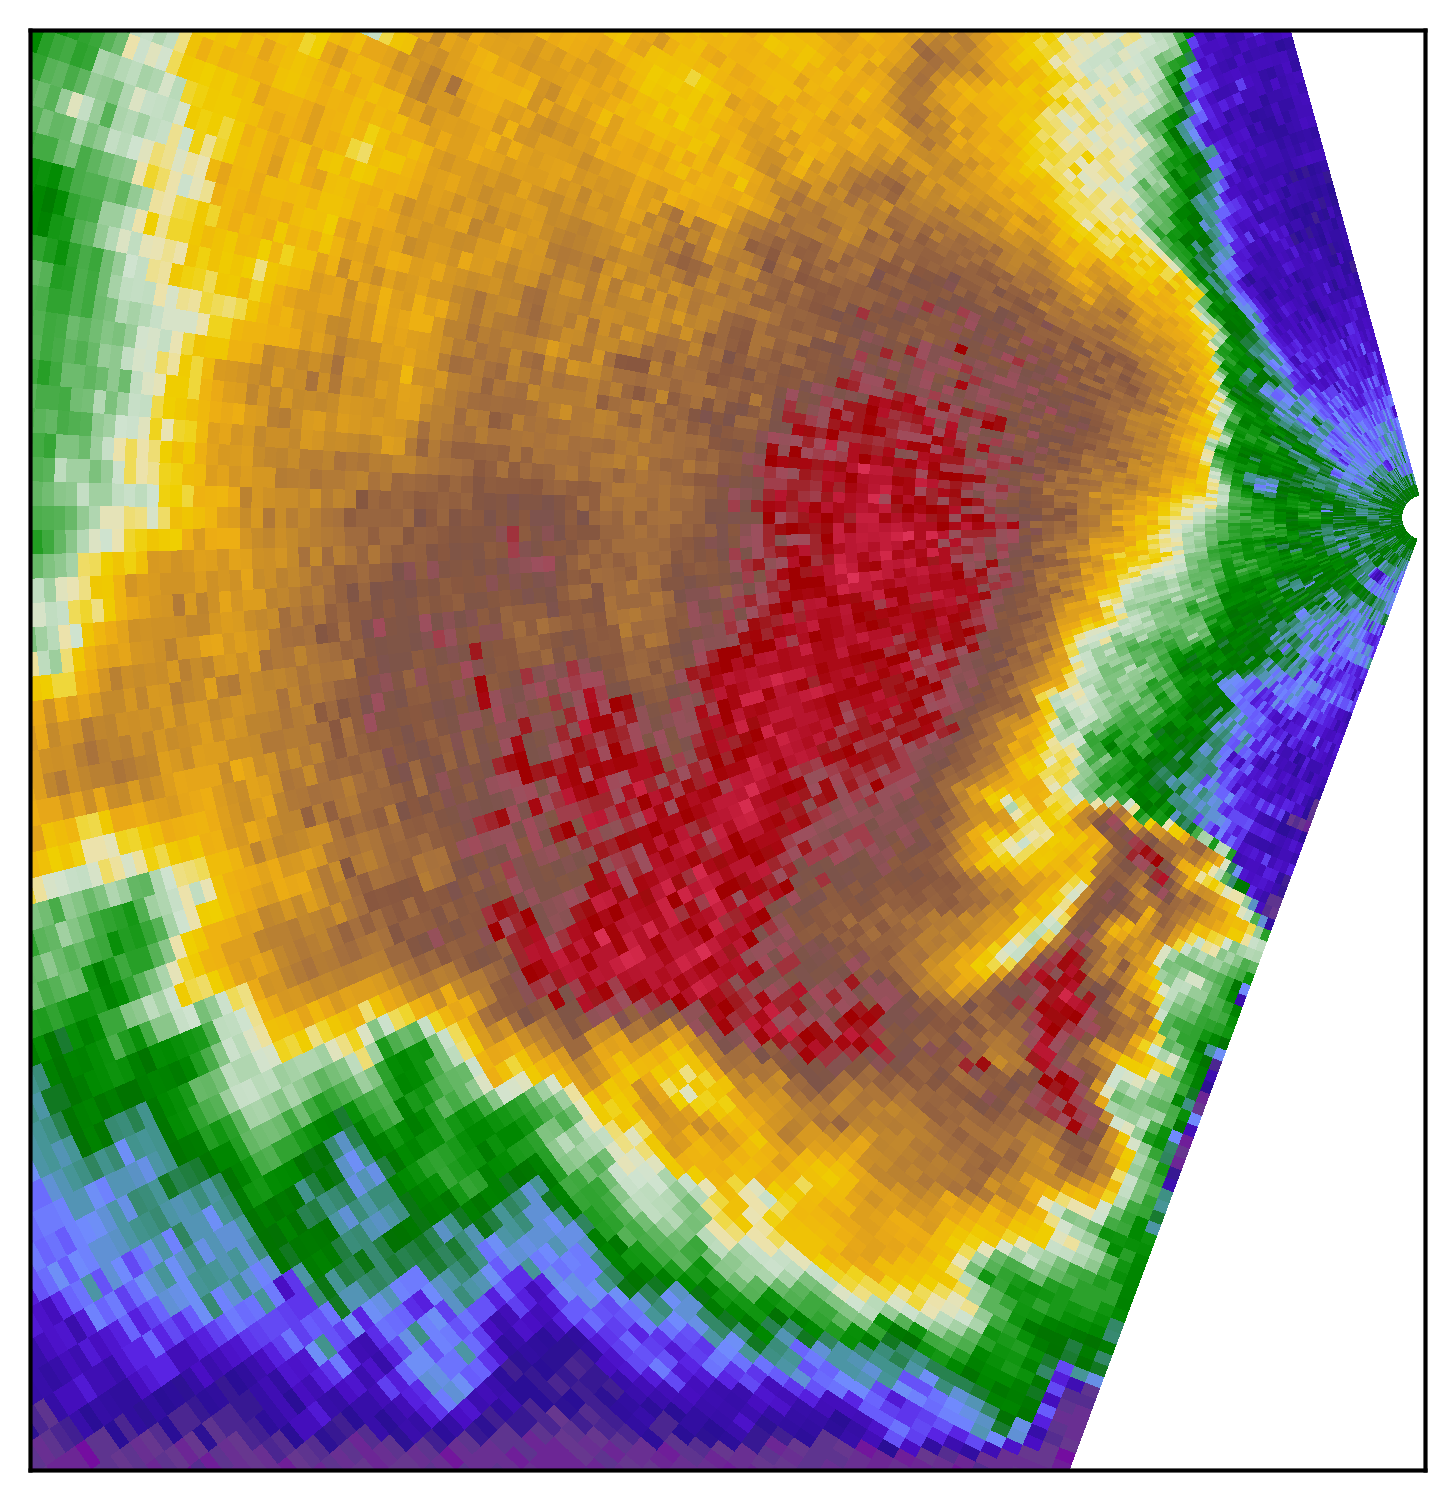
\includegraphics[scale=0.17]{figures/title_ppi.png}}
\logo{
\includegraphics[scale=0.6]{figures/eec_logo_black.png}}

%Python is known for having “batteries included”: a feature-filled standard
%library which reduces development effort for many common tasks, such as logging,
%configuration files, and command line parsing. The utilization of this standard
%library allows the addition of features to software while adding little
%additional code, or even reducing the amount of code for existing software.
%Also, by virtue of its dynamic nature and powerful built-in data structures,
%Python is able to provide a drastically simpler interface for reading NetCDF
%datasets compared to the standard interfaces in languages like C or FORTRAN.
%Python's concept of modules additionally facilitates the creation of small,
%reusable software components, which promotes code reuse. These qualities reduce
%the volume of code that must be developed and maintained, which accelerates the
%development cycle. The porting of a software radar simulator from pure C to a
%mixture of C and Python is used as a case study in the benefits moving software
%to Python.

\begin{document}

\frame{\titlepage}

\section[Outline]{}
\begin{frame}{Outline}
    \tableofcontents
\end{frame}

\section{Background}
\begin{frame}
  \frametitle{Simulation Software}
  \begin{itemize}
    \item Software simulates radar data from numerical simulation output
    \item Radar data simulated based on configured radar and scanning strategy parameters
    \item Computationally expensive simulation
    \item Desire to utilize as a teaching tool -> EEK! Other USERS!
    \item Before: 5400 LOC C
    \item Now: 2000 LOC Python, 2900 LOC C (+8500 LOC FORTRAN Library)
    \item Time to "python-ize": ~3 months for a single graduate student (me)
  \end{itemize}
\end{frame}

\begin{frame}
  \frametitle{Why I Chose Python}
  \begin{itemize}
    \item Simple Syntax
    \item Powerful built-in data structures
    \item Excellent string manipulation
    \item Strong built-in library
    \item NumPy - array math
    \item SciPy - scientific algorithms
    \item Matplotlib - plotting
  \end{itemize}
\end{frame}

\section{Batteries Included...The Standard Library}

\begin{frame}
  \frametitle{Why is the Standard Library Important?}
  \begin{itemize}
    \item Libraries you can count on with every installation -> minimal dependency headaches
    \item Starting point for finding solid libraries to handle given tasks
    \item Some examples
      \begin{itemize}
        \item re - Regular Expressions
        \item bz2, zipfile, gzip - compressed file handling
        \item os - OS-independent ways for working with files
        \item os.path - OS-independent path/file-name manipulation
        \item subprocess - Running other programs
        \item datetime - working with dates and times
        \item ConfigParse - configuration file parsing
        \item optparse - command-line option parsing
        \item logging - controlling output
      \end{itemize}
    \item TODO: HIGHLIGHT LAST 3 ABOVE
  \end{itemize}
\end{frame}

\begin{frame}
  \frametitle{Configuration Files}
  \begin{itemize}
    \item The radar simulation software makes use of configuration files to
      control various radar operation parameters
    \item Made use of ConfigParse module from the standard library
    \item Provides flexible configuration files with support for sections and comments
    \item Simple API to open a configuration file and begin reading options
  \end{itemize}
\end{frame}

\begin{frame}
  \frametitle{Configuration Files:Impacts}
  \begin{itemize}
    \item Replaced brittle file format with something that is easy for users to understand
    \item OLD FORMAT HERE
    \item NEW FORMAT HERE
    \item Replaced brittle, unmaintainable code with something much easier to enhance
    \item Shrank code by 600 LOC
  \end{itemize}
  HUGE usability improvment.
\end{frame}

\begin{frame}
  \frametitle{Command Line Parser}
  \begin{itemize}
    \item optparse module included in Python standard library
    \item Handle parsing of commandline into passed in arguments and options
    \item EXAMPLE COMMANDLINE
    \item EXAMPLE COMPLEX COMMANDLINE
    \item Programmatically add individual options
    \item EXAMPLE CODE HERE
    \item Can also set default values for options
    \item Get a help display for free
    \item SHOW HELP SCREEN HERE
  \end{itemize}
\end{frame}

\begin{frame}
  \frametitle{Command Line Parser:Impacts}
  \begin{itemize}
    \item Increased code by 100 LOC
    \item However, old code was simplistic
    \item Those 100 lines of new code added support for:
    \begin{itemize}
      \item Controlling how many message are written to screen
      \item Controlling detail of messages
      \item Logging messages to file
      \item Drastically improved help message
    \end{itemize}
  \end{itemize}
  Overall impact was a large increase in usability with minimal development effort.
\end{frame}

\begin{frame}
  \frametitle{Logging}
  \begin{itemize}
    \item Printing messages to the console is necessary to keep tabs on the program.
    \item However, the messages that are useful to me as a developer are not the
      same as what other users needs to see.
    \item Logging libraries provide custom printing functions that allow fine-grained
      control of what messages are printed
    \item Python includes the logging module that includes a raft of features:
    \begin{itemize}
      \item Control of message information (time, filename, line number, etc.)
      \item Different message commands for different levels (warning, info, debug, etc.)
      \item Different message handlers (write to file, write to screen, email?)
    \end{itemize}
  \end{itemize}
\end{frame}

\begin{frame}
  \frametitle{Logging:Impacts}
  \begin{itemize}
    \item Added 40 LOC to set up logging, replaced prints with logger.*
    \item Gained the ability to get detailed messages with a simple command line flag
    \item Gained the ability to only turn on some messages when \emph{I} want them
    \item No \#ifdefs or commenting/uncommenting prints
    \item Big improvements in usability for me as a developer and for other users
  \end{itemize}
\end{frame}

\section{NetCDF}

\begin{frame}
  \frametitle{Python NetCDF API}
  \begin{itemize}
    \item Many packages:
    \begin{itemize}
      \item PyNIO - Part of NCAR's PyNGL package
      \item Scientific.IO.NetCDF (?)
      \item Pupynere
      \item NetCDF4
    \end{itemize}
    \item But they all pretty much follow the same API
    \item Which is \emph{much} simpler than reading and writing NetCDF in C
  \end{itemize}
\end{frame}

\begin{frame}
  \frametitle{Comparison: Reading a variable}
  TODO: Need code samples from C and Python for reading a variable (without error handling)
\end{frame}

\begin{frame}
  \frametitle{Comparison: Writing an attribute}
  TODO: Need code samples from C and Python for writing a string attribute on the file (without error handling)
\end{frame}

\begin{frame}
  \frametitle{Python NetCDF API: Impacts}
  \begin{itemize}
    \item Rewrote I/O layer -- shrank by 800 LOC
    \item Better output metadata
    \item Adding new fields and attributes much simpler with Python
    \item As a consequence, the output files contain much more useful
      information for reproducing previous results
  \end{itemize}
\end{frame}

\section{Wrapping existing code}

\begin{frame}
  \begin{itemize}
    \item Ctypes - wrap existing library objects (dll's on Windows, .so's on UNIX)
    \item F2Py - call fortran functions from Python
    \item Cython - Generate C-code (and compiled library) from Python-like syntax
  \end{itemize}
  TODO: HIGHLIGHT Ctypes and F2Py above?
\end{frame}

\section{Modularity}

\begin{frame}
  \begin{itemize}
    \item Integration of existing python scattering code
    \item Same code used to generate plots for other analyses
    \item Re-use leads to better testing
  \end{itemize}
\end{frame}

\section{Wrapping up}

\begin{frame}
  \frametitle{Concluding remarks}
  \begin{itemize}
    \item Python offers many built-in libraries that can simplify development...
    \item or allow you to implement features you never would have tried
    \item Python can \emph{drastically} simplify working with NetCDF files
    \item Python allows you keep your performance sensitive code while giving you
      flexibility for those parts that don't need speed (usually most of your code)
    \item Python reduces development time for many things--at a cost of run-time
  \end{itemize}
\end{frame}

\begin{frame}
  \frametitle{Thanks and Questions}
  Thanks to:
  INSERT NUMPY, MATPLOTLIB, PYTHON, SCIPY here
  Questions?
\end{frame}

\end{document}
